
\section{HAR en Android}
\begin{frame}{HARDroid}

\framesubtitle{HAR en Android}

\setbeamercovered{transparent}
\begin{columns}

\column{0.4\textwidth}
\begin{itemize}
\item \textbf{HARDroid} 
\begin{itemize}
\item Servicio Reconocedor
\item Clasificador din�mico
\end{itemize}
\begin{spacing}{0.5}

\pause{}
\end{spacing}
\item \textbf{ActivitySurvey}
\begin{itemize}
\item Cliente de Reconocimiento
\item Encuesta guiada
\end{itemize}
\begin{spacing}{0.5}

\pause{}
\end{spacing}
\item \textbf{Backend C4.5} 
\begin{itemize}
\item Servicio web de recolecci�n
\item Aprendizaje en-linea
\end{itemize}
\end{itemize}

\column{0.6\textwidth}
\begin{overprint}
\onslide<1> 
\begin{center}
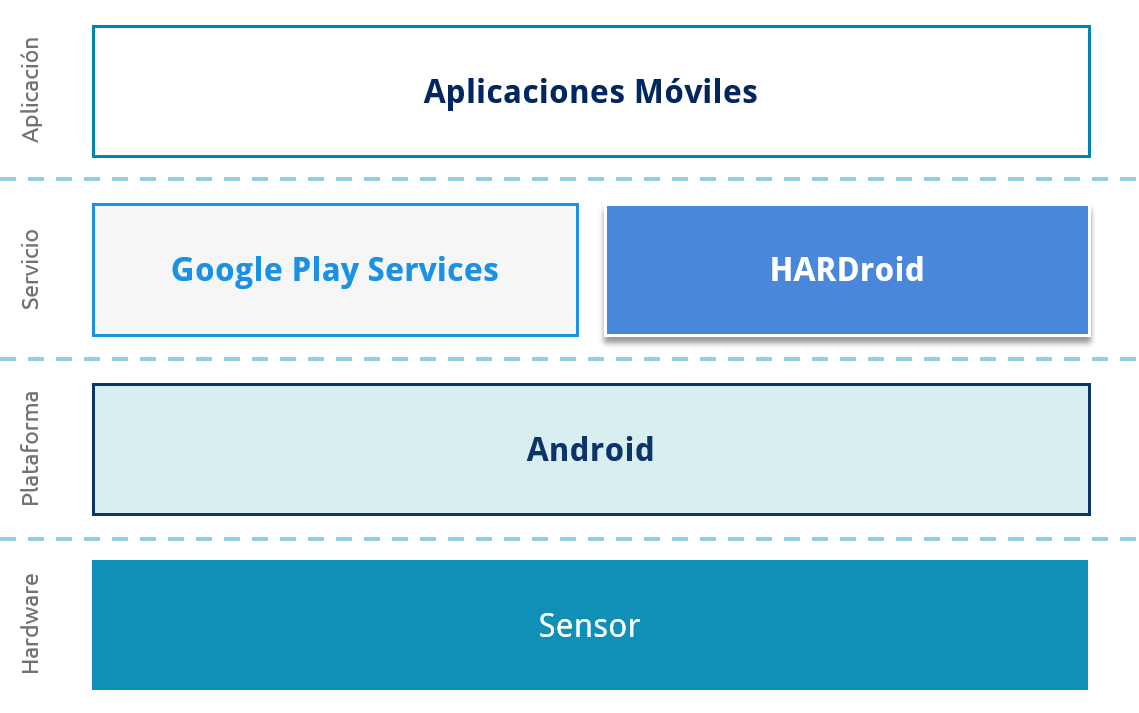
\includegraphics[width=1\columnwidth]{propuesta/graphics/hardroid_stack1}
\par\end{center}
\onslide<2> 
\begin{center}
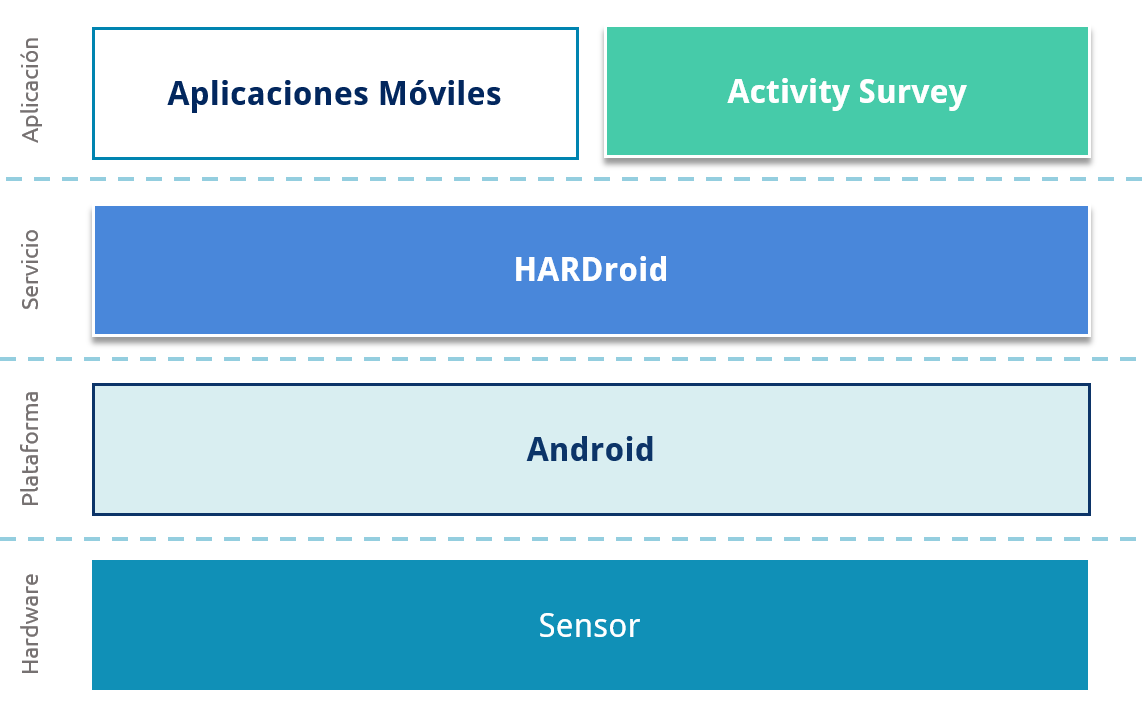
\includegraphics[width=1\columnwidth]{propuesta/graphics/hardroid_stack2}
\par\end{center}
\onslide<3> 
\begin{center}
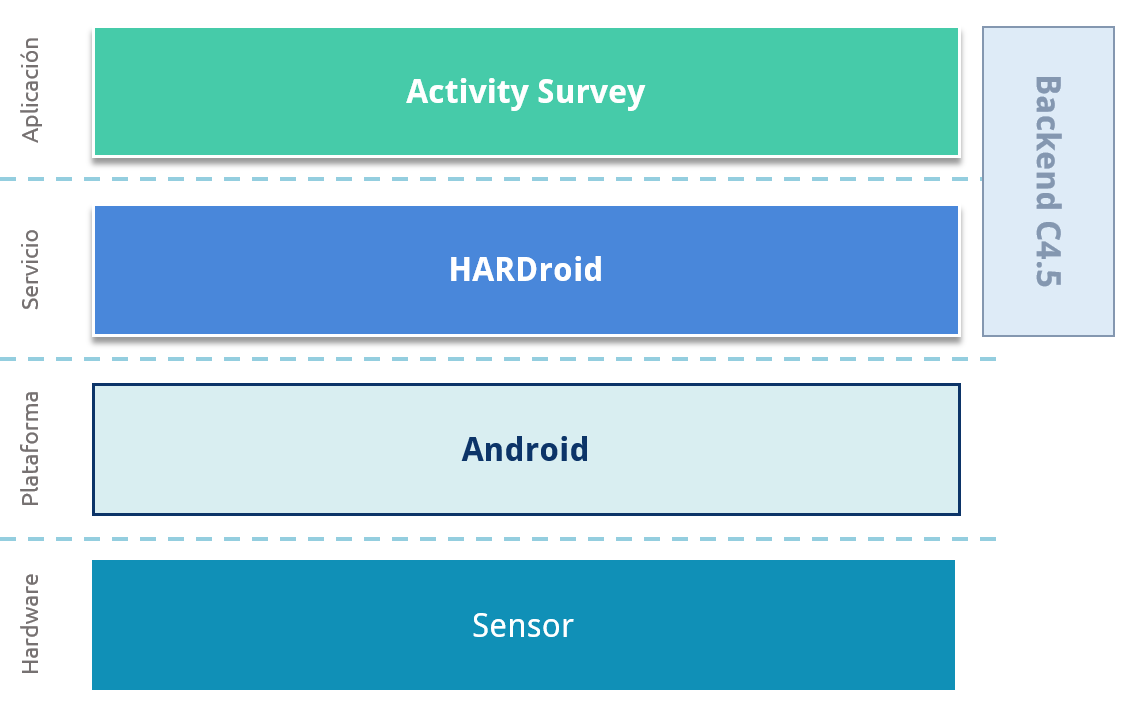
\includegraphics[width=1\columnwidth]{propuesta/graphics/hardroid_stack3}
\par\end{center}

\end{overprint}
\end{columns}

\end{frame}
%
\begin{frame}{HARDroid Colaborativo}

\framesubtitle{HAR en Android}
\begin{center}
\begin{figure}
\begin{centering}
\caption{Proceso colaborativo de mejora continua}
\par\end{centering}
\begin{overprint}
\onslide<1> 
\begin{centering}
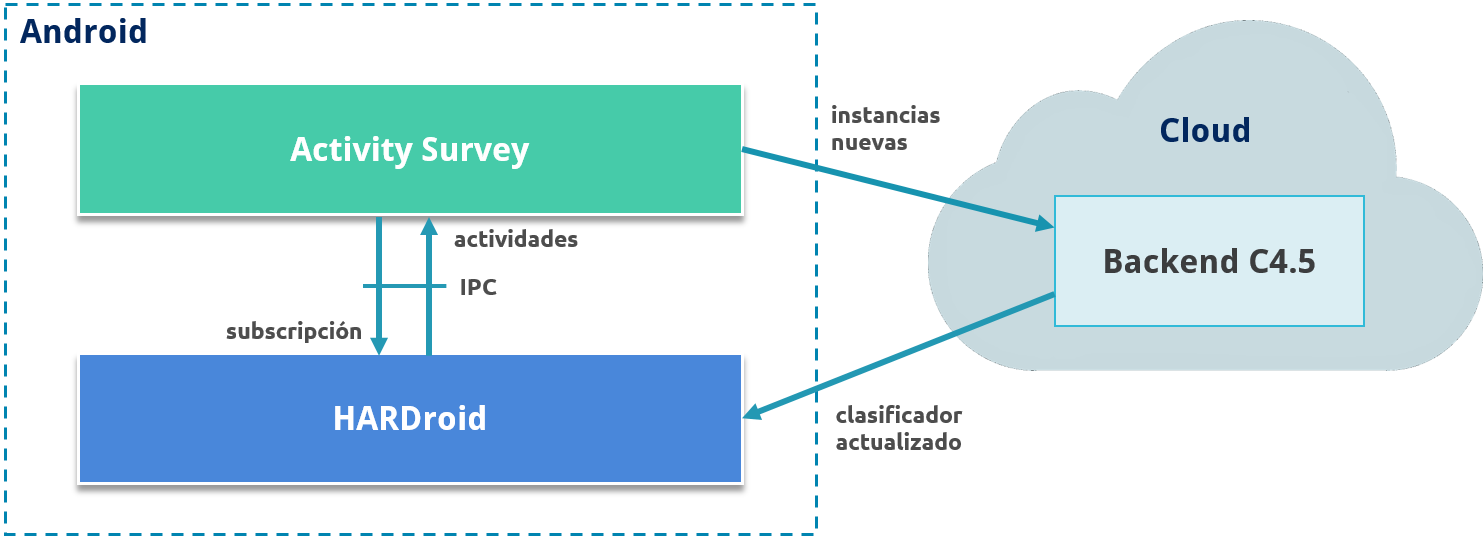
\includegraphics[width=1\columnwidth]{propuesta/graphics/hardroid_colab1}
\par\end{centering}
\onslide<2> 
\begin{centering}
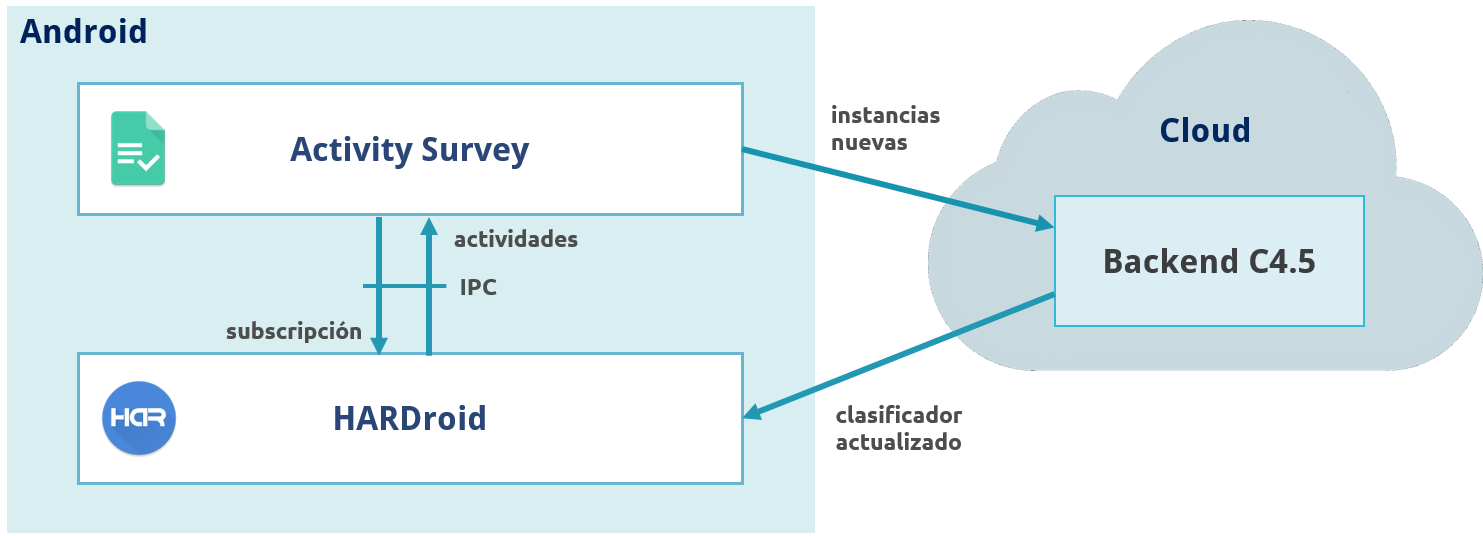
\includegraphics[width=1\columnwidth]{propuesta/graphics/hardroid_colab2}
\par\end{centering}
\centering{}\emph{Disponible en} \structure{\begin{center}
Google Play Store
\par\end{center}}
\end{overprint}
\end{figure}
\par\end{center}
\end{frame}

